%!TEX root = ../template.tex
%%%%%%%%%%%%%%%%%%%%%%%%%%%%%%%%%%%%%%%%%%%%%%%%%%%%%%%%%%%%%%%%%%%
%% chapter5.tex
%% UNIPD thesis document file
%%
%% Chapter with introduction
%%%%%%%%%%%%%%%%%%%%%%%%%%%%%%%%%%%%%%%%%%%%%%%%%%%%%%%%%%%%%%%%%%%

\typeout{NT FILE chapter5.tex}%

\chapter{Progettazione e Implementazione di un Sistema di Streaming Audio}
\label{cha:streamingaudio}

\prependtographicspath{{Chapters/Figures/Covers/}}

Le soluzioni commerciali proposte da marchi rinomati come Sonos, Marshall e Bose richiederebbero l'installazione di collegamenti cablati in ogni sezione dell'edificio, rappresentando inoltre una scelta onerosa in termini di costi. Inoltre, la centralizzazione di questi sistemi da un singolo server si è dimostrata problematica. Per superare queste sfide, viene proposto un approccio wireless innovativo, in cui un server primario è incaricato di distribuire file audio pre registrati ai diversi client presenti nella rete.

Il sistema proposto deve soddisfare tre requisiti fondamentali. Primo, è necessaria una stretta dipendenza tra le librerie del server primario e dei client. Secondo, occorre una connessione internet robusta o una rete locale, con il server principale configurato con un indirizzo IP statico. Terzo, l'intera architettura deve essere economicamente vantaggiosa, semplificando sia l'implementazione che la manutenzione.

Per realizzare questo progetto, si è scelto di utilizzare il Raspberry Pi, un microcomputer con il supporto del sistema operativo Linux. Dopo ulteriori ricerche, è stata selezionata la versione DietPi, basata su Debian, preferendola ad altre versioni con \gls{gui}. Sono stati quindi considerati due possibili approcci di implementazione: uno basato su Balena Sound con sistema operativo Balena e l'altro impiegando i server Mopidy e Snapcast su DietPi.

Questa introduzione pone le basi per una discussione dettagliata su come realizzare un sistema di comunicazione audio efficiente e scalabile in un ambiente educativo distribuito, affrontando sfide pratiche con soluzioni tecnologiche innovative.

\section{Architettuera del Sistema}
\noindent

Il progetto richiede un ecosistema completo che permetta di trasformare un tradizionale sistema di altoparlanti cablati in un sistema wireless. Gli altoparlanti devono poter comunicare con il server principale, che consente la trasmissione di musica o file audio richiesti dal cliente. Per implementare questo sistema, è stato scelto un hardware compatibile con Linux, come il Raspberry Pi (nello specifico il Zero 2w), utilizzando il sistema operativo DietPi per ottimizzare l’uso della memoria cache della CPU e della memoria Ram.

Snapcast è stato installato sia sul server che sui client, permettendo una trasmissione audio sincronizzata multi-room tra i dispositivi. \cite{snapcast}

Per consentire l’accesso remoto al server e la gestione della riproduzione musicale, è stato implementato Mopidy \cite{mopidy}, un server musicale versatile. In quale offre diverse estensioni, come Mopidy-File, Mopidy-Iris e Mopidy-Mobile, che facilitano l’accesso e la gestione dei file musicali presenti nella directory locale e/o server designata. Insieme a Mopidy, è stato installato anche \gls{mpd} per creare un ambiente di riproduzione musicale virtuale, che consente l’accesso remoto attraverso interfacce come Iris (frontend) o \gls{mobile}. Con queste estensioni, è possibile eseguire i comandi basici come riproduzione, mettere in pausa e regolare il volume. Il controllo del volume dell’intero gruppo di altoparlanti è possibile solo se Snapcast è abilitato e in esecuzione come servizio.

\begin{figure}[h]
    \centering
    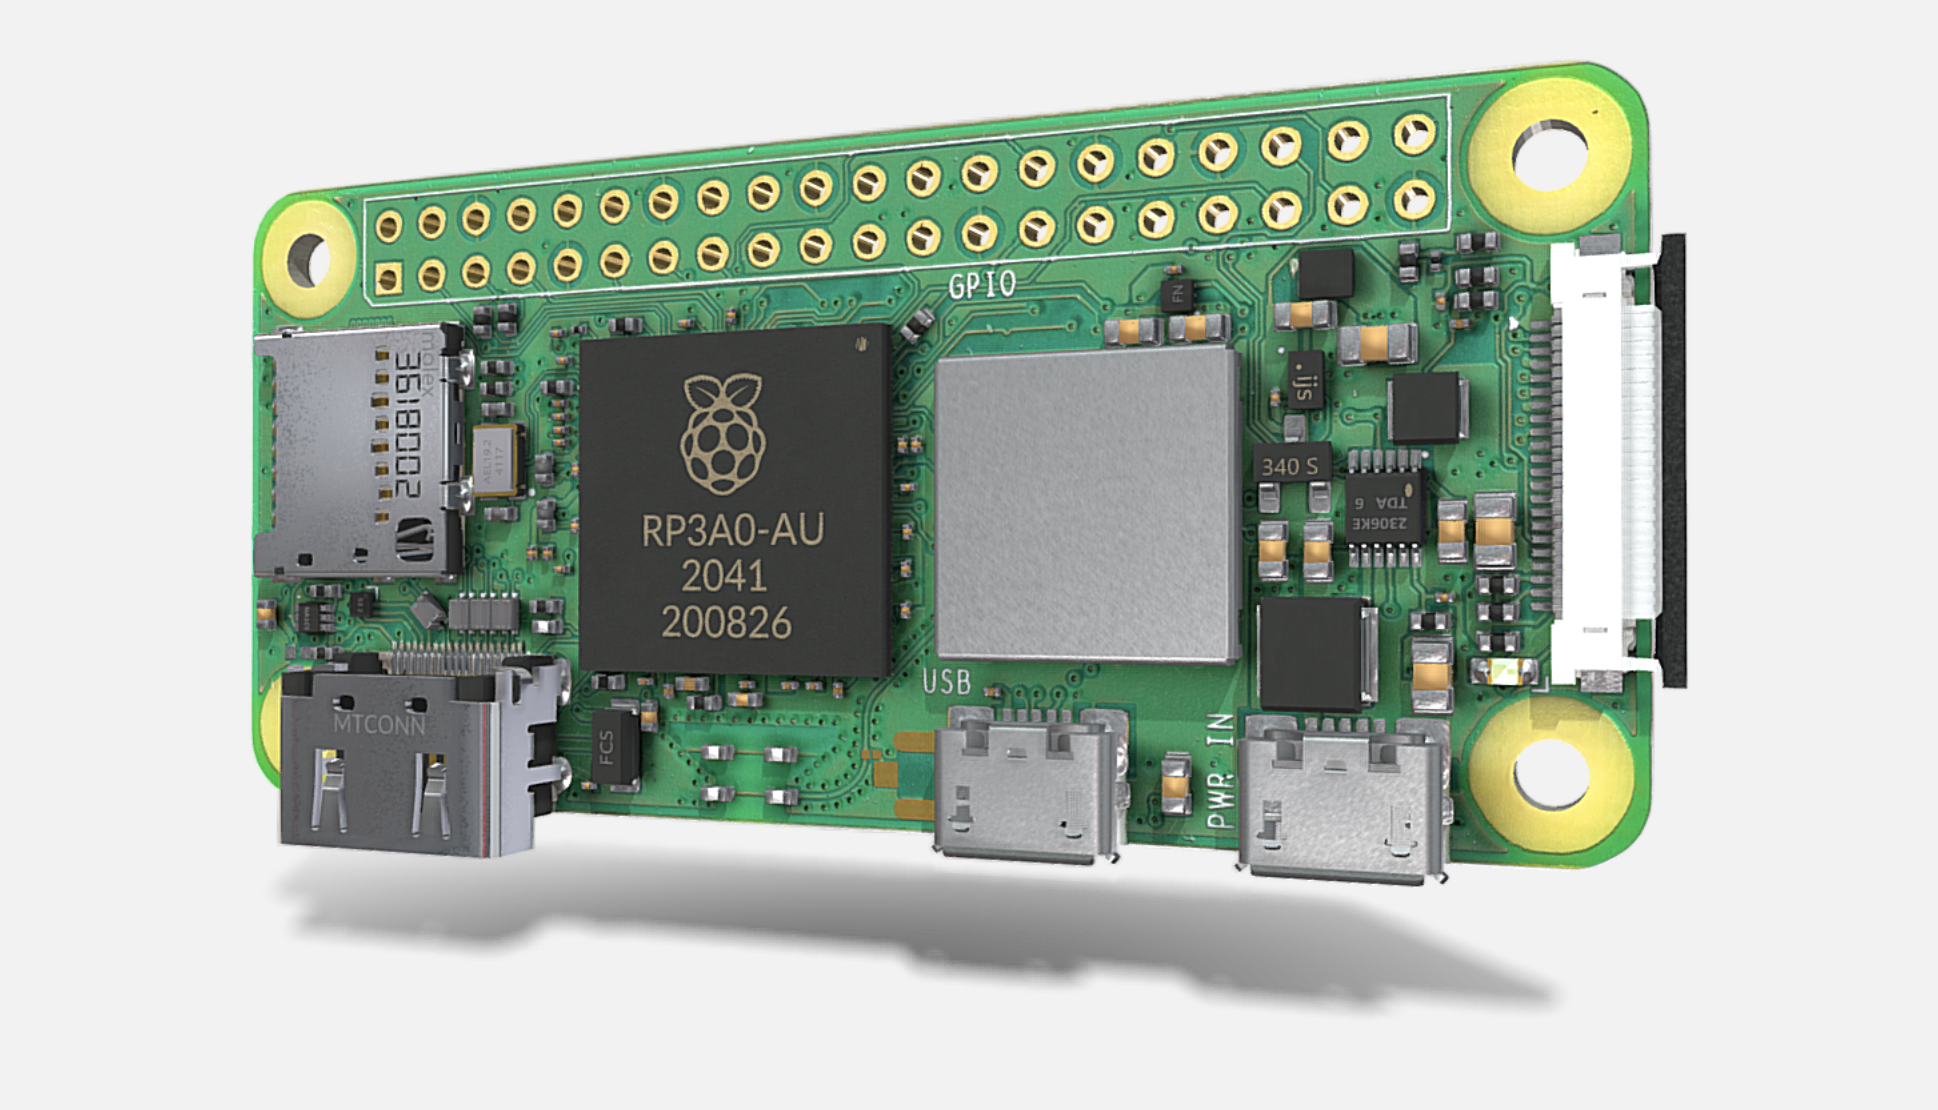
\includegraphics[width=0.5\textwidth]{Chapters/Figures/3d_render_2w.png}
    \caption{\small Raspberry Pi Zero 2w 3d render.} 
    \label{fig:zero2w_3d_render}
\end{figure}

\begin{comment}

\begin{figure}[h]
    \centering
    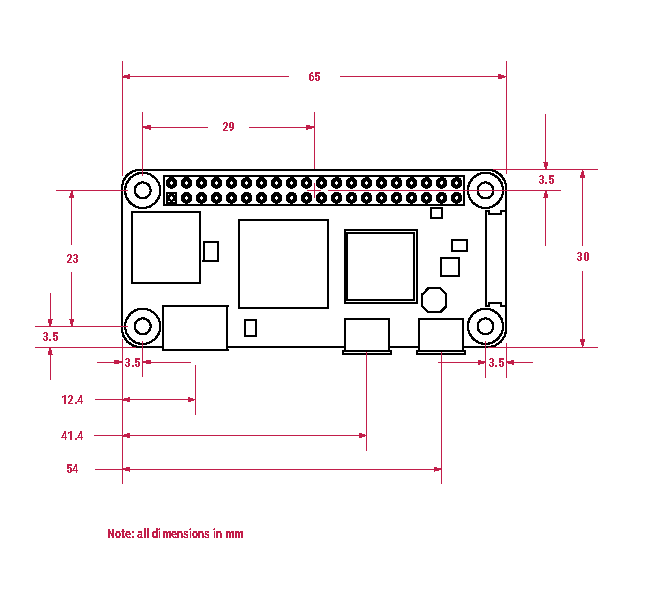
\includegraphics[width=0.6\textwidth]{Chapters/Figures/mechanical_scheme_2w.pdf}
    \caption{\small Raspberry Pi Zero 2w mechanical scheme. \cite{parallax}} 
    \label{fig:zero2w_mechanical_scheme}
\end{figure}

\end{comment}
